
\chapter{Basic Reinforcement Learning Example Using Logistic Regression }
\label{chapter:logistic-regression}

Logistic Regression is one of the methods that can be used as an activation function. Others include Rectified Linear Units (ReLU) and the Perceptron. In classification the conceptual target of using this activation function is to achieve the all mighty goal of linear separability. In RL we are more concerned with constructing a reasonable function approximator for the state or action value function. In classification it can be common to a sigmoid function on the final layer to calculate the probability the input is of a particular class. This function is shown in Figure~\ref{figure:logistic-function}. This function limits our possible value function output to be between $0$ and $1$, I have found that it is better to at least use the \textit{tanh} function with a range in the $-1$ to $1$ range (see Figure~\ref{figure:tanh-function}).

\begin{figure}
	\centering
	\label{figure:logistic-function}
	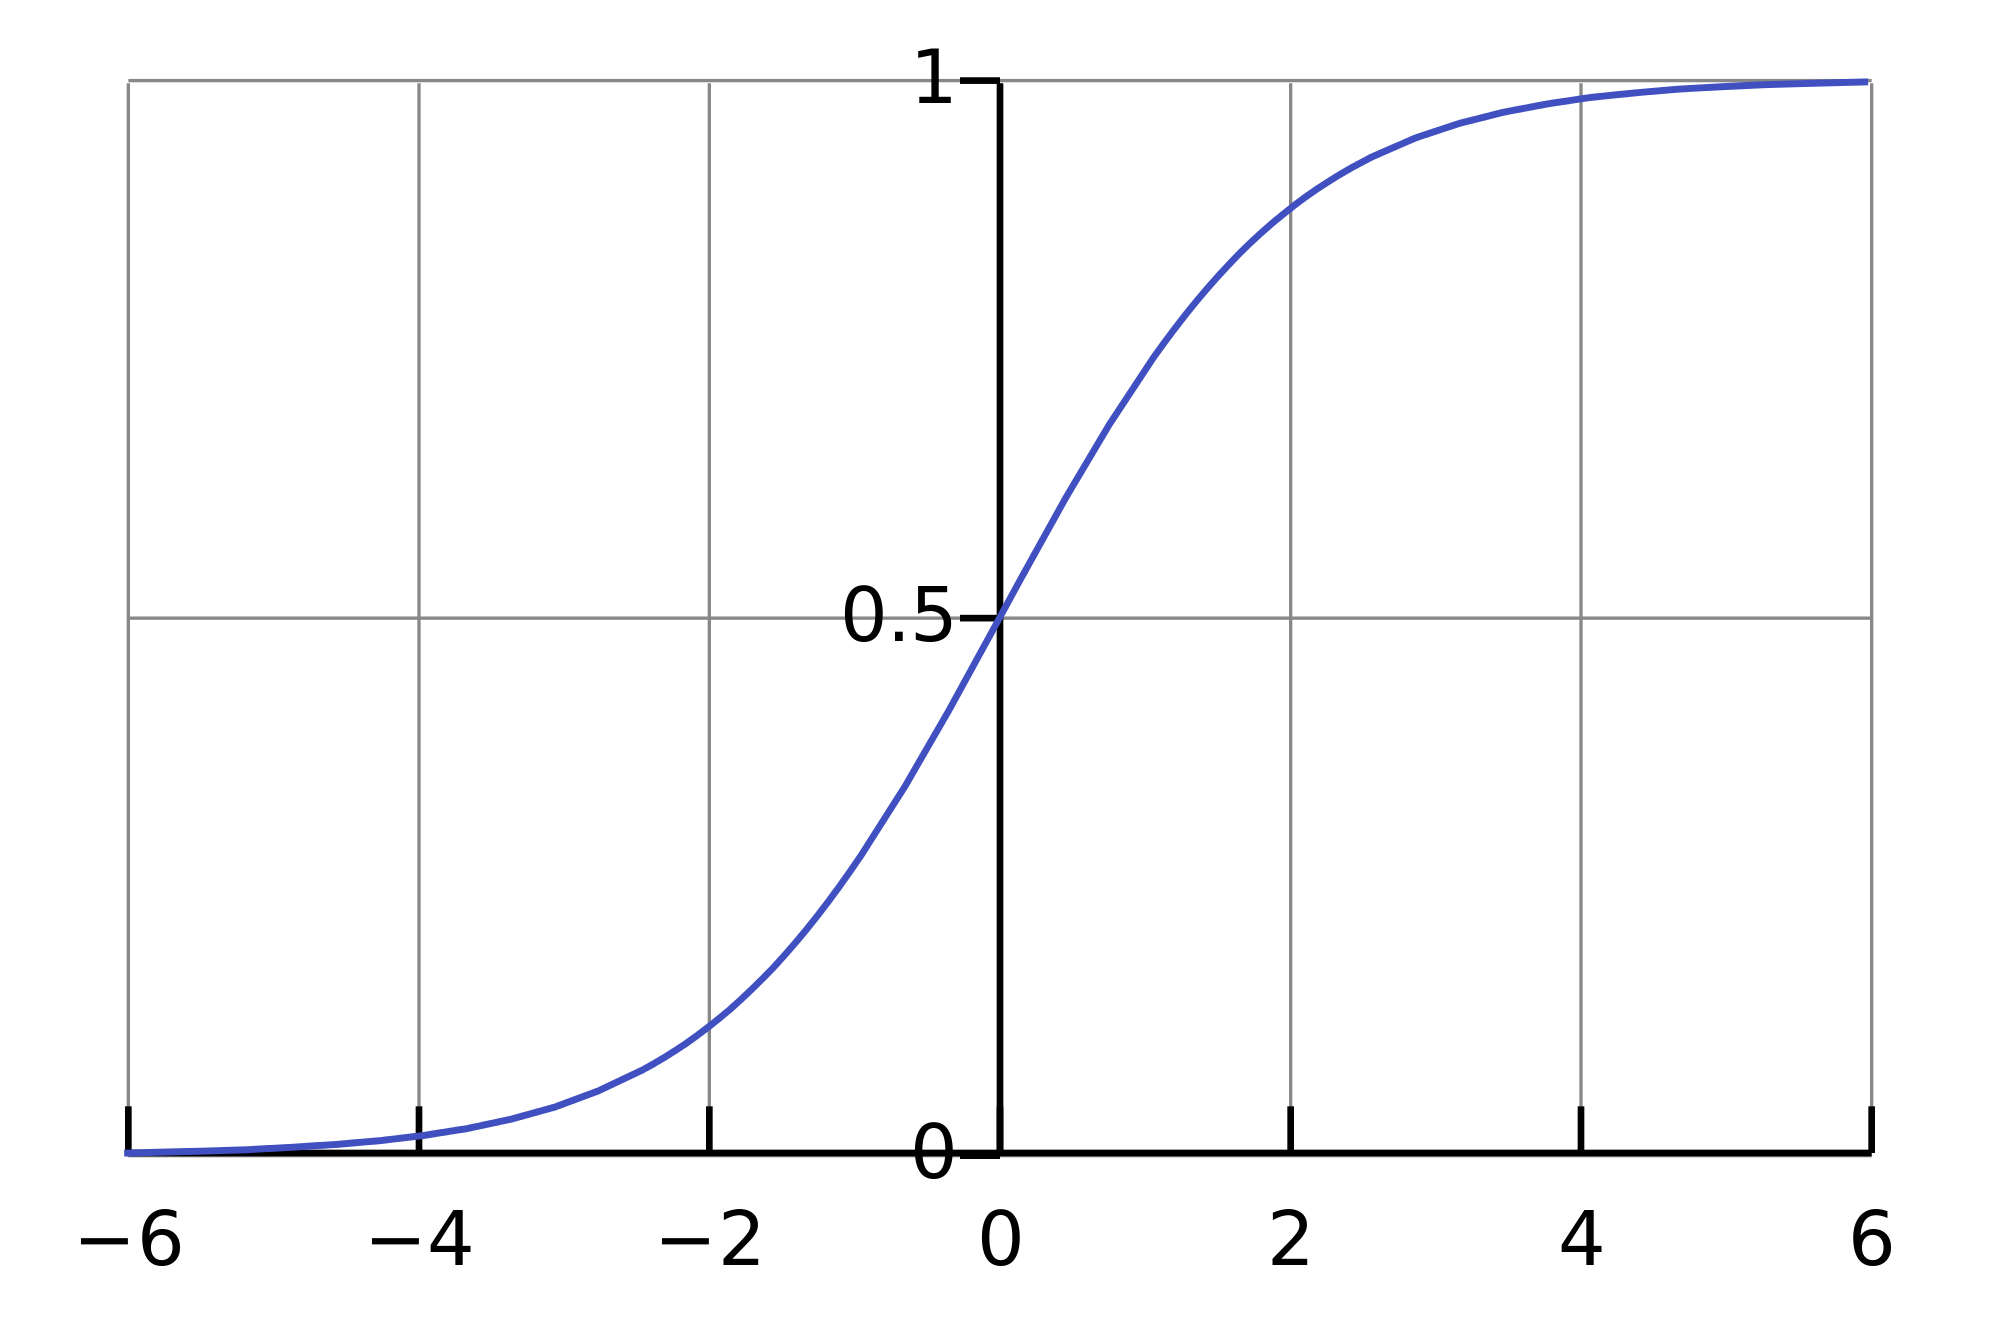
\includegraphics[width=0.95\linewidth]{../images/Logistic-curve.png}
	\caption{A graph of the logistic function.}
\end{figure}

\begin{equation}
% 	sigmoid(\inputVector,\weightMatrix,\basisVector)=\frac{1}{1+e^{-\weightMatrix\inputVector+\basisVector}}
	sigmoid(\inputVector)=\frac{1}{1+e^{-\inputVector}}
\end{equation}  

\begin{figure}
	\centering
	\label{figure:tanh-function}
	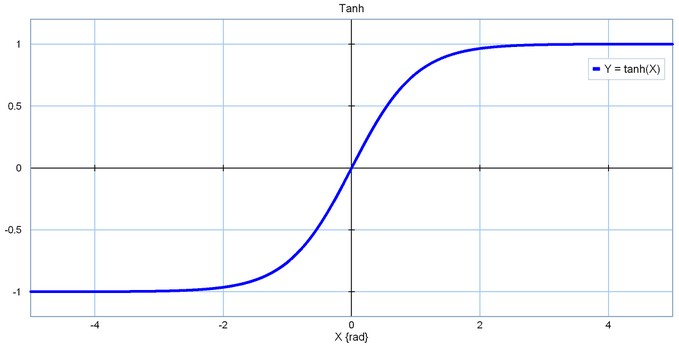
\includegraphics[width=0.95\linewidth]{../images/tanh_zoom60.jpg}
	\caption{A graph of the tanh function.}
\end{figure}

\begin{equation}
	tanh(\inputVector)=\frac
	{e^{\inputVector}-e^{-\inputVector}}
	{e^{\inputVector}+e^{-\inputVector}}
	%tanh(\inputVector,\weightMatrix,\basisVector)=\frac
	%{e^{\weightMatrix\inputVector+\basisVector}-e^{-\weightMatrix\inputVector+\basisVector}}
	%{e^{\weightMatrix\inputVector+\basisVector}+e^{-\weightMatrix\inputVector+\basisVector}}
\end{equation}


Often in RL the parameters of the model are denoted as \modelParameters and the goal is to optimize the bellman error with respect to these parameters. For logistic regression using the \textit{tanh} activation function this translates to $\modelParameters=\{\weightMatrix,\basisVector\}$. Where \weightMatrix are the weights for the model and \basisVector is a bias for the model. Somewhat similar to the more common $y=mx+b$ for defining a line. The \basisVector effectively shifts the curve to the right or left.

\section{Multidimensional Regression}

This model extends to multiple dimensions or \textit{actions} rather easily, $\inputVector, \basisVector$ become vectors and \weightMatrix is now a matrix with dimensions $len(\inputVector) x numActions$. Then the sigmoid function returns a vector of Q-values, one for each action in state \inputVector. The optimal action using the Q-Learning method can then be computed as

\begin{equation}
\action^{*}= \argmax_{\action}\qValueFunction{\state}{\action}{}= \argmax_{i} tanh(\state,\theta)
\end{equation}
Keep in mind that in the multidimensional case $tanh(x,\theta)$ returns a vector with a length equal to the number of actions for the actor. The index with the maximum value is chosen $\argmax tanh(x,\theta)$ and corresponds to the index for the best action to execute in state \state,

\subsection{Model Optimization}

To perform optimization using a tanh model a cost function is needed. The cost function is used to compute the difference between the current model and the perfect solution. For RL we use the Bellman Error to determine this
\begin{equation}
cost(R, S, S') = sum(0.5 * \delta(R, S, S')^{2})
\end{equation}
This cost function gives a fair measure of the model error. Note, in this formulation R,S,S′ are vectors or matrices and the squared the cost is used so that positive and negative errors to not cancel each other out in the sum. It is also common to use mean in this function instead of sum because sum is effected more by variable scale. Including our model in the cost function gives
\begin{equation}
cost(R, S, S', \theta) = sum(0.5 * \delta(R, S, S', \theta)^{2})
\end{equation}

To determine in what direction along the cost function contour will result in less error the gradient wrt the model parameters is needed 
$\frac{\partial cost}{\partial \modelParameters}$ in this case $\frac{\partial cost}{\partial \weightMatrix}, \frac{\partial cost}{\partial \basisVector}$ . This can be calculated in Theano rather easily.

\begin{lstlisting}
    g_W = T.grad(cost=cost, wrt=model.W)
    g_b = T.grad(cost=cost, wrt=model.b)
\end{lstlisting}

With the gradient in hand we can make a update rule to step in the direction of less cost.
\begin{equation}
	\weightMatrix' = \weightMatrix + (-\frac{\partial cost}{\partial \weightMatrix} \learningRate), 
	\basisVector' = \basisVector = (-\frac{\partial cost}{\partial \basisVector} \learningRate)
\end{equation} 

This can also be done in Theano rather simply as 

\begin{lstlisting}
updates = [(model.W, model.W + (-g_W * learning_rate),
           (model.b, model.b + (-g_b * learning_rate)]
\end{lstlisting}


Those are the steps needed to perform common Stochastic Gradient Descent (SGD). It should be noted that the \textit{learning rate} \learningRate for RL problems should be rather small, the effect of this will be discussed and shown later.

\subsection{Model Training}

Every time the agent selects an action \action in some state \state that leads to receiving some reward \reward and resulting in a new states \nextState experience is gained. This single tuple of experience is put in an experience history that is used to improve the model training. The experience history serves a similar purpose as training data in classification problems. 
Training the model (or updates) is done over a mini batch, where a mini batch is a randomly selected sample from the experience history of the agent. 

\subsection{Action Selection and Exploration}

A common method to select an action to execute is \eGreedy action selection. This algorithm simply selects one of the available actions at random with probability $\epsilon$. Otherwise, the selected action comes from the policy \policyFunction{\state}{}, in this case the logistic regression model.

\subsection{Learning Rate}

One tough challenge that has only recently seen good solutions is dealing with highly erratic policy changes. The policy can swing from one end of the spectrum to the other making it almost impossible for the optimization to eventually settle on a good policy.
Earlier, I said we would look at the effect the learning rate has on the learning process. The learning rate is one of the parameters that influences the erraticness of the policy. The effect of a learning rate that is to high is shown in the Figure~\ref{figure:erratic-policy}. Focus on the policy on the right that describes the optimal action/direction to be selected when the agent is in the location on the map that is the location of the arrow.

\begin{figure}
	\centering
	\label{figure:erratic-policy}
	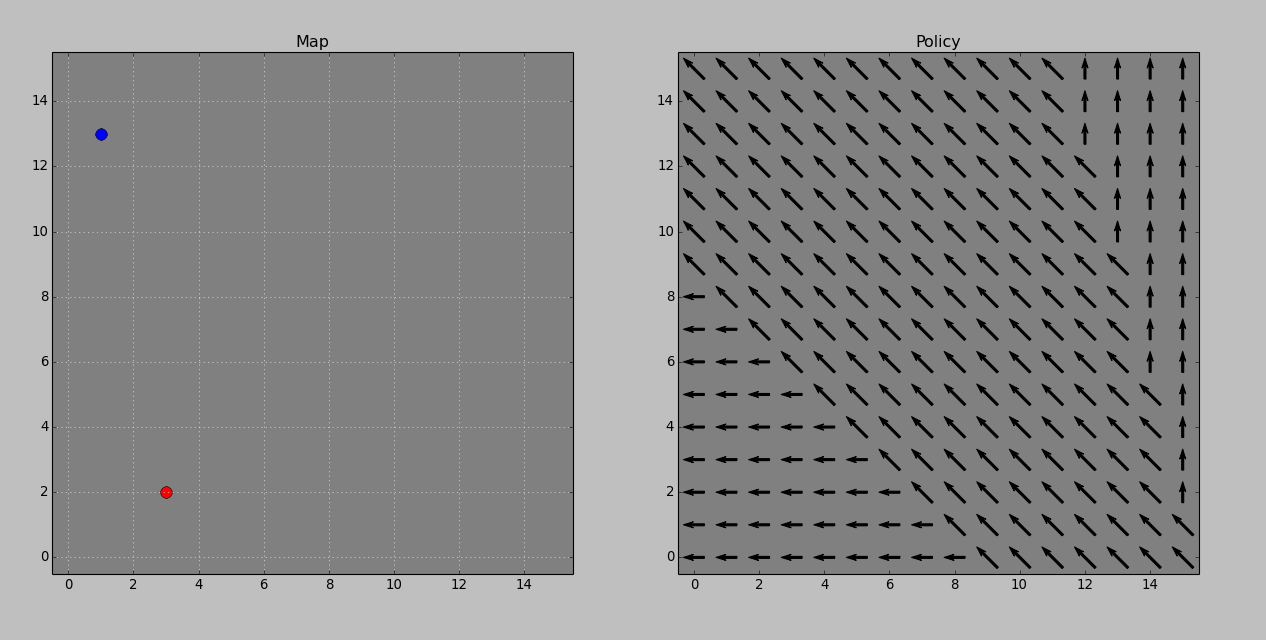
\includegraphics[width=0.9\linewidth]{../images/before_policyJump.png}
	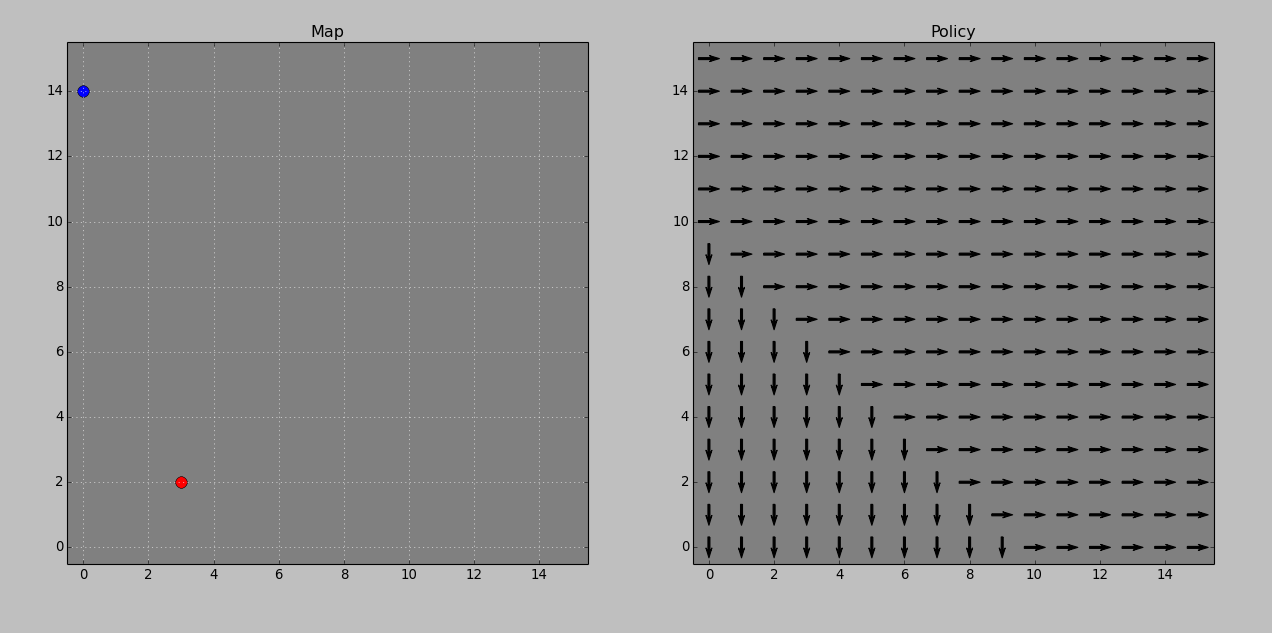
\includegraphics[width=0.9\linewidth]{../images/after_policyJump.png}
	\caption{These two figures show the change in the policy after a single training update. 
	This significant change is the result of a learning rate with a high value.}
\end{figure}

After lowering the learning rate from 0.5 to 0.01 small manageable policy updates are made, as can be seen in Figure~\ref{figure:smooth-policy}.

\begin{figure}
	\centering
	\label{figure:smooth-policy}
	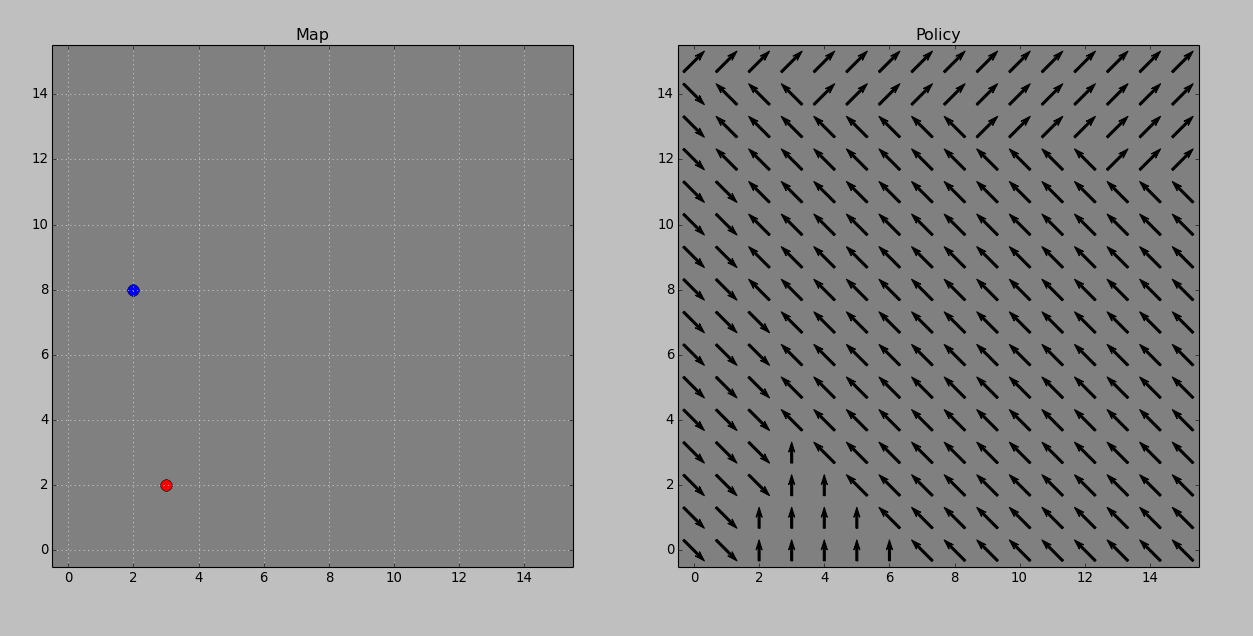
\includegraphics[width=0.9\linewidth]{../images/before_policyJump-lower-learningRate.png}
	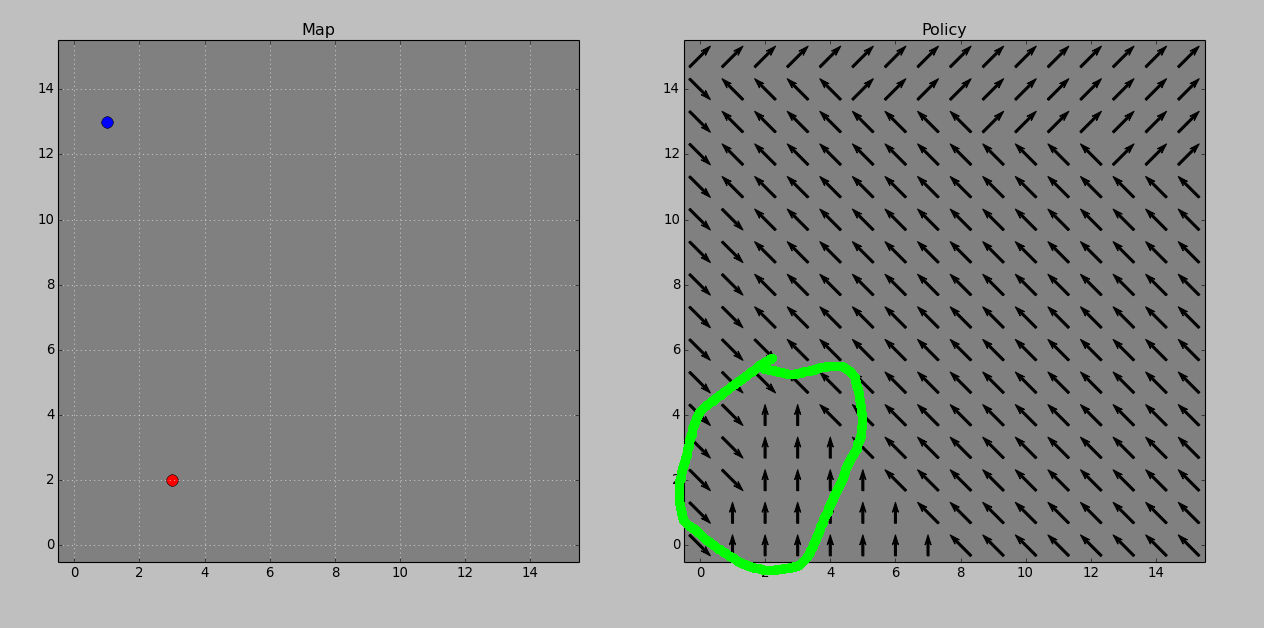
\includegraphics[width=0.9\linewidth]{../images/after_policyJump-lower-learningRate.png}
	\caption{These two figures show the change in the policy after a single training update. 
	With respect to Figure~\ref{figure:erratic-policy} the policy updates are much smaller and smoother.}
\end{figure}

The Code 
Can be found here.

\begin{comment}
References:
1. https://en.wikipedia.org/wiki/Activation_function 
2. https://en.wikipedia.org/wiki/Q-learning 
3. http://deeplearning.net/software/theano/tutorial/examples.html#logistic-function 
4. http://deeplearning.net/tutorial/logreg.html#logreg 
5. https://webdocs.cs.ualberta.ca/~sutton/book/ebook/the-book.html 
\end{comment}